% Template for computer science thesis at the TU Munich
% Authors Benedikt Mas y Parareda, Johannes Becker, Gunnar Schroeder, Elmar Juergens

\documentclass[11pt,a4paper]{book}

\usepackage{multicol}
\usepackage[latin1]{inputenc}
\usepackage{amsmath,amssymb,amsfonts,amsthm}
\usepackage{graphicx}
\usepackage{rotating}
\usepackage{url}
\usepackage{latexsym}
\usepackage{makeidx}
\usepackage[usenames,dvipsnames]{color}
\usepackage[english,german]{babel}

\usepackage{longtable}

%maybe temporary packages: 
\usepackage{color}

\makeindex

\usepackage{geometry,mflogo,xspace,texnames,path,booktabs,bm}
\usepackage[hyperindex,bookmarks,pdfborder=0,plainpages=false,pdfpagelabels]{hyperref}
\usepackage{subfigure}
\usepackage{listings}
\usepackage{footnote}

\usepackage[nonumberlist,nopostdot,nomain,toc,acronym]{glossaries}
\makeglossaries

%Settings applicable to the complete document

%Breaks URLs properly and draws them in a nice font
\urlstyle{sm}

\renewcommand{\ttdefault}{pcr} % Courier has a bold shape, default tt does not


%Include a CVS revision number in the document
\def\version$#1 #2 #3 #4${#3}
\newcommand{\CVSrevision}
{\version$Id: thesis.tex 00 2010-07- 18:32:21Z Elmar $}


%Decrease the default indentation of paragraphs
\parindent=0.3cm

%new or changed commands
\renewcommand\contentsname{Table of Contents}
\newcommand{\chapref}[1]{Chapter~\ref{#1}}
\newcommand{\secref}[1]{Section~\ref{#1}}
\newcommand{\appref}[1]{Appendix~\ref{#1}}
\newcommand{\figref}[2][]{Figure~\ref{#2}#1}
\newcommand{\listref}[2][]{Listing~\ref{#2}#1}
\newcommand{\tabref}[2][]{Table~\ref{#2}#1}
\newcommand{\acroref}[1]{List of Abbreviations~\ref{#1}}

\newcommand{\etal}{et al.\ }
\newcommand{\ie}{i.\,e.\ }
\newcommand{\eg}{e.\,g.\ }
\newcommand{\gap}{\hspace{1.5cm}}

\newcommand{\dotcup}{\ensuremath{\mathaccent\cdot\cup}}

\renewcommand\lstlistingname{Listing}
\renewcommand\lstlistlistingname{List of Listings}

\renewcommand\contentsname{Table of Contents}

%hyphenation rules
\hyphenation{ele-ments}
\hyphenation{Composite-Expression}
\hyphenation{dia-gram}

% footnote stuff....
\makesavenoteenv{tabular} 

% set listings to texttt
\lstset{language=Java}

%%%%%%%%%%%%%%%%%%%%%%%%%%%%%%%
%
% THE DOCUMENT
%
%%%%%%%%%%%%%%%%%%%%%%%%%%%%%%%
\begin{document}
\bibliographystyle{alpha}

%Title Page
\frontmatter
\pagestyle{empty}

\begin{center}
\begin{Huge}
Fakult\"aten f\"ur Informatik 
\end{Huge}
\vspace{0.3in}
\begin{Huge}
und Maschinenwesen
\end{Huge}

\vspace{0.4in}
\begin{huge}
der Technischen Universit\"at M\"unchen
\end{huge}\\
%\vspace{1.2in}
%\vspace{2in}\\
%\vspace{1.2in}
\vspace{4cm}
\begin{LARGE}
Interdisziplin\"ares Projekt
\vspace{4cm}
\end{LARGE}\\


\begin{Huge}
Model Transformations for Product-Service Systems
\vspace{3cm}
%Coupled Evolution of\\Metamodels and Models \vspace{1.2in}

\end{Huge}
\begin{LARGE}
Bernhard Radke, Konstantin Govedarski \vspace{0.6in}
\end{LARGE}
%
%\begin{Large}
%Bachelor's Thesis in Computer Science
%\vspace{1.2in}
%
%\end{Large}
\end{center}
%Title Page
\frontmatter
\pagestyle{empty}

\begin{titlepage}
\begin{center}
\begin{huge}
Fakult\"aten f\"ur Informatik und Maschinenwesen
\end{huge}\\
\vspace{4mm}
\begin{Large}
der Technischen Universit\"at M\"unchen
\end{Large}\\
\vspace{2.5cm}
\begin{Large}
Interdisziplin\"ares Projekt
\vspace{2.75cm}
\end{Large}\\
\begin{huge}
Model Transformations for\\\vspace{5mm} Product-Service Systems
\end{huge}\\
\vspace{1.25cm}
\begin{large}
\begin{tabular}{ll}
\vspace{0.1in}
Verfasser:& Bernhard Radke\\
\vspace{0.2in}
& Konstantin Govedarski\\
\vspace{0.2in}
Aufgabensteller:&Prof. Dr.-Ing. Udo Lindemann\\
\vspace{0.1in}
Betreuer: &Christopher M\"unzberg\\	
\vspace{0.1in}
&Daniel Kammerl\\
\vspace{0.1in}
&Konstantin Kernschmidt\\
\vspace{0.2in}
&Thomas Wolfenstetter\\
Submission Date:&28.04.2014\end{tabular}
\end{large}
\end{center}

%Version stuff
%\begin{flushright}
%\begin{tiny}
%Version: \CVSrevision\\
%Date: \today
%\end{tiny}
%\end{flushright}

\end{titlepage}

%\input{declaration.tex}
%\input{abstract.tex}
%\input{abstract-de.tex}
%\input{acknowledgement.tex}


% Table of Contents
\setcounter{tocdepth}{2}                % Sets depth of table of contents. 0 is chapter, 1 is sections, 2 is subsections
\setcounter{secnumdepth}{2}             % Sets depth of numbering of toc contents

\selectlanguage{english}
\tableofcontents


%List of Figures
%TODO ENABLE
%\listoffigures

%List of Tables
%\listoftables

%List of Listings
%\lstlistoflistings

\newacronym{PSS}{PSS}{Product-Service System}
\newacronym{PSSIF}{PSS-IF}{Product-Service System Integration Framework}
\newacronym{poc}{PoC}{Proof of Concept}
\newacronym{dsl}{DSL}{Domain-Specific Language}
\newacronym{xml}{XML}{Extensible Markup Language}
\newacronym{xslt}{XSLT}{EXtensible Stylesheet Language Transformations}
\newacronym{api}{API}{Application Programming Interface}
\newacronym{xmi}{XMI}{XML Metadata Interchange}
\newacronym{emf}{EMF}{Eclipse Modeling Framework}
\newacronym{xsd}{XSD}{XML Schema Definition}
\newacronym{sysml}{SysML}{Systems Modeling Language}
\printglossary[title=List of Abbreviations,type=acronym]

\mainmatter
\pagestyle{headings}


% Chapters. Each one in its own file

\chapter{Introduction}
\label{chap:intro}

In present-day economic circumstances, businesses are presented with numerous challenges. Some of those challenges originate from the businesses themselves, like for example the strategic aim of growing and expanding into new markets, or the forging of customer and market awareness. Other challenges originate from the business and regulatory environment of the business in question. These environments force a business to be even more competitive and to optimize for sustainability. To achieve this, industries no longer put the product itself at the core. Rather, they incorporate the product into a number of services, which reach from the lowest-level technical detail to the highest-level customer interaction and provide for optimal product utilization. In this sense, what a company tries to sell nowadays is not just the product itself, but a service through which the customer consumes the product, while being isolated from technical detail and unnecessary responsibility. Such a complete solution is defined by \cite{ref:schenkl} as a \gls{PSS}.

While the incorporation of Product-Service Systems in an industry requires an initial effort and an evolution of the companies' cultures, it can lead to a more concise and efficient utilization of resources to the benefit of both the companies themselves and their customers. 

\section*{Importance of Integration}

After their implementation and market introduction, Product-Service Systems can bring numerous benefits to a company. Nevertheless, their implementation brings a number of challenges with regards to communication, integration and complexity. To illustrate this, consider the parties involved in the development and production cycles of a \gls{PSS}. Both development and production involve a number of disciplines, each acquainted with its own modelling languages and tools. Each of these \glspl{dsl}, furthermore, is concerned only with those aspects of the overall systems, which are relevant for the discipline at hand. As a result, each involved party has only a limited excerpt of the entire \gls{PSS} at its disposal. In the worst case, this leads to contradictions in the design and implementation of the system. In the moderate case, it only incurs significant synchronization and management costs to the company. It is thus of crucial importance for the success of a PSS venture to establish a mechanism though which the models developed by different disciplines can be transformed to each other, or even to incorporate them all in a single model, representing the \gls{PSS} in its entirety.

\section*{PSS Integration Framework}

An approach to the integration of the disciplines involved in the development of a \gls{PSS} is researched jointly in the SFB 768 (\cite{ref:sfb}). The approach is named \gls{PSSIF} \cite{ref:paper} and provides a methodology and semantics for bringing the business, computer science and mechanical engineering aspects of a \gls{PSS} together. In its core, the framework describes a common structure which is sufficiently expressive to incorporate the \gls{PSS}-wide relevant features of each domain-specific aspect of the PSS. This structure is depicted in \figref{fig:canonic}.

\begin{figure}
\centering
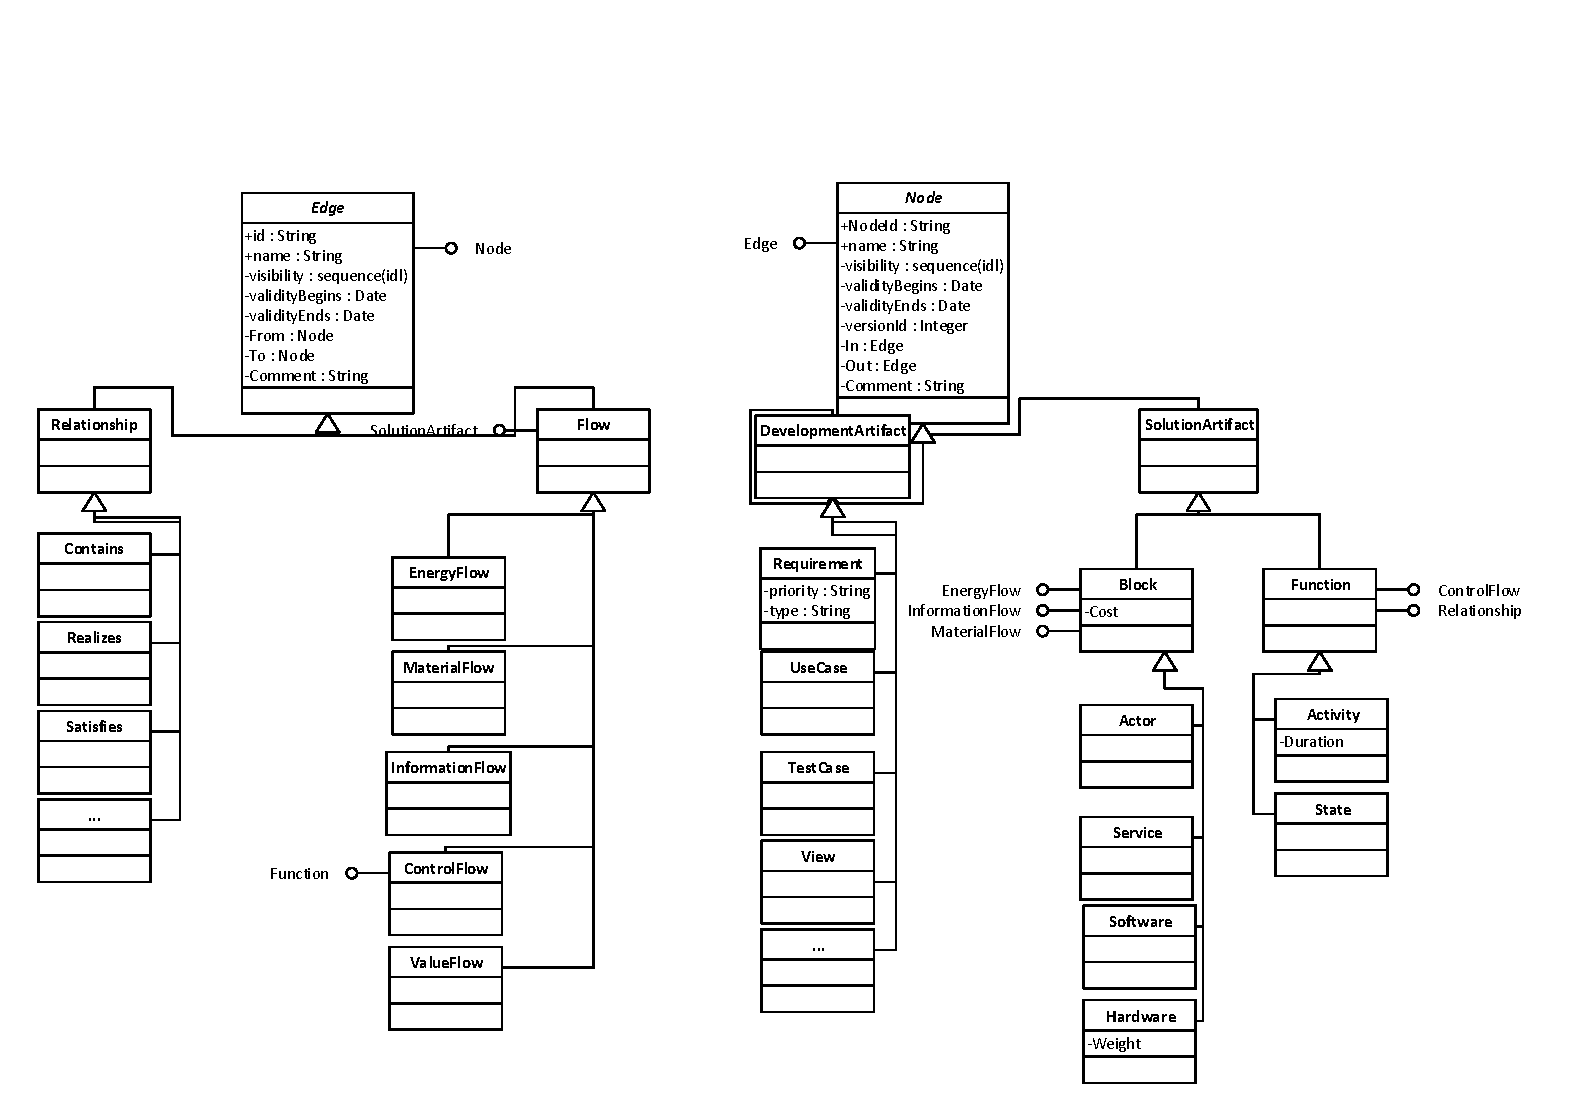
\includegraphics[width=\textwidth]{figures/PSSIF.pdf}
\caption{PSS-Integration Framework Common Structure}
\label{fig:canonic}
\end{figure}

The main goal of the \gls{PSSIF} is the usage of this structure for the integration of models of different disciplines. For this purpose, a key step is the ability to translate models from and to this common structure.

\section*{Scope of the Interdisciplinary Project}

In the context of the \gls{PSSIF}, the goal is to design and implement a \gls{poc} software utility which:

\begin{itemize}
\item follows the PSS-IF methodology and semantics,
\item can transform a model described in one relevant domain-specific language into another relevant \gls{dsl},
\item considers the following domain-specific languages relevant:
	\begin{itemize}
	\item Event-driven Process Chain (EPC) Diagrams \cite{ref:epk}
	\item Business Process Model and Notation (BPMN) Diagrams \cite{ref:bpmn}
	\item Flow-oriented Functional Modeling (FFM) Diagrams \cite{ref:ufm} modelled using the Soley-Tool (formerly known as BOOGGIE) \cite{ref:soley}
	\item Systems Modeling Language for Mechatronics (SysML4Mechatronics) Diagrams \cite{ref:sysml} and,
	\end{itemize}
\item should, at the time of its delivery, support at least two of the relevant domain-specific languages.
\end{itemize} 

\section*{Structure of this Documentation}
In \chapref{chap:approach} we discuss possible approaches to the conceptual structure of the \gls{poc} developed in this interdisciplinary project. \chapref{chap:impl} describes the implementation of the \gls{poc}. The results obtained from the \gls{poc} are described in \chapref{chap:results}. In {\chapref{chap:outlook} we provide a few ideas about possible future developments on the basis of the provided \gls{poc}.



%\chapter{Requirements}
\label{chap:req}

TODO

\begin{itemize}
\item classification of requirements
\item listing of requirements to the thingie
\item keep in mind scope of the research topic
\end{itemize}
\chapter{Approach}
\label{chap:approach}

This chapter presents and justifies the approach of the \gls{poc} software utility developed in the scope of this interdisciplinary project. A comparison of different transformation methods is provided in \secref{sec:approach:transform}. Thereafter, the chosen approach to the realization of model transformations is defined on an abstract level in \secref{sec:approach:pssif}.

\section{Transformation Methods}
\label{sec:approach:transform}

Provided with the task to transform between different Models, there is an number of possible solutions. These can roughly be categorized into direct and indirect transformation methods.

\subsection{Direct Transformation Methods}

Direct transformation methods are such which define rules for the transcription from source to destination \gls{dsl} directly, i.e. such methods do not produce a (defined) intermediate result, but rather are always language-specific. Furthermore, it is possible to differentiate between syntax-dependent and syntax-independent technical solutions for this kind of transformations.

\subsubsection{Syntax-Dependent Transformations}

Syntax-dependent transformations build upon a technology which is well-suited for processing the syntax of the source and destination \glspl{dsl}. For example, considering \glspl{dsl} which both use the \gls{xml}\cite{ref:xml} as their concrete syntax, an appropriate transformation technology is \gls{xslt}\cite{ref:xslt}.

\subsubsection{Syntax-Independent Transformations}

Syntax-independent direct transformation methods are a category of methods, which, while still transforming directly from a source \gls{dsl} to a destination \gls{dsl}, are not coupled to the concrete syntax of any particular \gls{dsl}. Such transformation approaches can be realized in a high-level programming language, which relies on a number of serialization and de-serialization components for the transmission of own language-specific data-structures to the respective \gls{dsl} concrete syntax serializations.

\subsection{Indirect Transformation Methods}

Indirect transformation methods are methods which rely on a stable and well defined intermediate format. A particular transformation between two \glspl{dsl} is performed by first transforming from the source DSL into the intermediate language and then transforming from the intermediate language to the target \gls{dsl}. From a technological perspective a differentiation between two categories of intermediate languages can be made: fixed and flexible intermediate languages.

\subsubsection{Fixed Intermediate Language Transformations}

Transformation methods with a fixed intermediate language can be realized in a high-level programming language. In this case the abstract syntax of the intermediate language is directly implemented as a data structure in the programming language. Thus, the intermediate language is described directly with the vocabulary of the programming language in use. Also, in this case, the transformations from and to \glspl{dsl} can be implemented directly in the syntax of the particular programming language, which makes it possible to utilize the language at its full expressiveness.

\subsubsection{Flexible Intermediate Language Transformation}

Transformation methods with a flexible intermediate language can also be technologically solved with a high-level programming language. As opposed to the previous case, here the intermediate transformation language is not fixed, in the sense that it is not hard-coded, but rather is a matter of configuration. Nevertheless, the intermediate language is still likely to be fixed for the scope of a single transformation.

\subsection{Discussion}

In this section the different transformation methods presented above are compared with each other. First, consider syntax-dependent transformation methods such as \gls{xslt}. On the one hand, this kind of transformations can be advantageous, because of their closeness to the languages at hand. A direct transformation can always be defined to enclose the maximum possible transmittable detail from one \gls{dsl} to another. On the other hand, such approaches impose a limitation to the entirety of languages which can be supported, due to their binding to the concrete syntax of those languages.

Syntax-independent direct transformations resolve this issue by abstracting the transformation description from the concrete syntax of the particular language, but still have a number of significant disadvantages. The most important one of these is the fact that such transformation methods require an explicit implementation for each pair of source and target \glspl{dsl}. As a result, with the introduction of each new language, a transformation procedure has to be defined for the combination of this language with every language already supported. Illustratively put, the result is a complete graph (each node being a \gls{dsl} and each edge a language-to-language transformation) and the number of necessary implementations grows exponentially in the number of \glspl{dsl} to support. In a dynamic field, where new languages may appear at any time, direct transformation approaches would thus incur significant costs on the longer run. Another disadvantage of these approaches is that with the growing number of transformation implementations, the code-base also grows proportionally. As a result, the code maintenance for such a utility also becomes more costly with time. 

To address the issue of exponentially growing complexity, indirect transformation methods can be used. As mentioned above, the methods in this category use an intermediate format to and from which transformations are made for each \gls{dsl}. As a result, the addition of a new \gls{dsl} will require the additional implementation of just one transformation, as opposed to as many transformations as there are languages to support. One solution in this case would be to directly implement the intermediate language in the programming language of choice. Such a description of the intermediate language and its transformation would, on the one hand, have the advantage of being expressed in the concepts of the used programming language and thus being accessible to any person with knowledge of this programming language. On the other hand, a fixed intermediate language is likely to be more costly once the evolution of the transformation framework is taken into consideration. In particular, any conceptual change in the intended meaning of a transformation would directly impact the transformations to and from all \gls{dsl} on the level of the programming language used. In essence, it would be necessary to potentially rewrite the code used for all transformations, which, considering a growing number of \glspl{dsl} and a continuously evolving modeling methodology, would once again incur long-term costs. Also, while the code base in this case is significantly smaller than in the case of direct transformation approaches, it still is growing in proportion with the number of \glspl{dsl} to support.

Finally, the most abstract approach is the usage of flexible intermediate language transformations. As opposed to the previous approach, here the intermediate language is not bound by concepts of the underlying programming language, but rather is only expressed in those concepts. As a result, the intermediate language can be defined on a level of abstraction on which most, if not all, new requirements can be expressed in terms of instantiation instead of code generation. In particular, only requirements which introduce new concepts to the language would require a modification of the code base. Requirements which merely imply a structural change only require a change in configuration. The advantages of such an approach are numerous, most importantly that it would provide a viable, flexible and powerful tool with only limited costs for the introduction of new \glspl{dsl}. The major disadvantage of such an approach is that it incurs a significant initial effort, as it requires the infrastructure for the description of the intermediate language to be implemented as well.

With this considerations made, the authors consider a flexible intermediate language approach to be the most appropriate one for the PoC software utility, as it best addresses the purposes of the PSS Integration Framework.

\section{The PSS-IF Transformation Method}
\label{sec:approach:pssif}

In the previous section the choice of a flexible intermediate language as a transformation method was made. In such a transformation method, there are a few central concepts, around which further definitions revolve.

\subsection{Levels of Meta}

In the following, we define the terms Metamodel and Model, as they are used within this documentation:

\paragraph{Model} A simplified description of reality, which only contains certain aspects of it, relevant for the creator of the model.\\

A model, while depicting certain aspects of reality, does not necessarily conform to any particular structure. The structure of a model is provided by a metamodel, defined as:

\paragraph{Metamodel} A description which defines how models are structured. A model is said to be an (ontological) instance of a metamodel, if the model structurally conforms to the metamodel.\\

No constraint is given to the number of meta-levels involved -- one can easily define meta-metamodels etc.

\subsection{Views and Viewpoints}

In the previous section the terms metamodel and model were defined. In this section we add the terms View and Viewpoint.

\paragraph{View} A view is a subset of a model.

\paragraph{Viewpoint} A viewpoint is a description which defines how views are created.\\

A viewpoint can thus be seen as a restricted or, more generally, transformed metamodel, which makes it possible to perceive model instances of this metamodel from a certain perspective (viewpoint). More precise definitions of this terms can be found in the ISO 42010 \cite{ref:42010} standard where the architecture description language refers to the \gls{PSSIF} metamodel, the architecture description to the \gls{PSSIF} model, the architecture viewpoint to the \gls{PSSIF} viewpoint and the architecture view to the \gls{PSSIF} view.

\subsection{PSS-IF in a Nutshell}
\label{sec:approach:pssif:nutshell}

Assume a metamodel describing all aspects of reality, which are of importance for the development of a \gls{PSS}. Such a metamodel is denoted as the PSS-IF Canonic Metamodel. For each \gls{dsl}, a viewpoint is defined on the basis of the PSS-IF Canonic Metamodel and captures only those parts of the canonic metamodel, which can be represented in the corresponding \gls{dsl}. Furthermore, viewpoints are defined in such a way that they can be used for both reading from and writing to a model.

This enables the achievement of a transformation between two exemplary \glspl{dsl} \textit{A} and \textit{B} through the following process:

\begin{enumerate}
\item Obtain the viewpoint for \gls{dsl} \textit{A}.
\item Create an empty model.
\item Add data to this model from an external source, whose abstract syntax is that of DSL \textit{A}.
\item Obtain a viewpoint for \gls{dsl} \textit{B}.
\item Create a new external target, conforming to the abstract syntax of \gls{dsl} \textit{B}.
\item Extract data from the model through the viewpoint for \gls{dsl} \textit{B} and write it to the target.
\end{enumerate}

After step 3 the model actually contains data conforming to the PSS-IF Canonic Metamodel. This is because the data is added through a viewpoint which internally transforms it to conform to the canonic metamodel. Therefore the data can, in step 6, be read directly with another viewpoint from the same model and is implicitly transformed to the abstract syntax of \gls{dsl} \textit{B}.

\subsection{Parts of the PSS-IF Proof of Concept}

To realize the PSS-IF transformation approach, a number of concepts need to be defined. While these concepts are briefly described here on an abstract level, they also closely resemble the implementation, presented in detail in the next chapter. The concepts required are provided in the following sections.

\subsubsection{PSS-IF Metamodel}

A PSS-IF Metamodel consists of a multitude of element types and data types. Each element type can be either a node type or an edge type. Both node and edge types can have attributes, and each attribute is bound to a particular data type. Associations between node types are defined through connection mappings, which are always bound to a certain edge type, i.e. an edge type can have multiple connection mappings, allowing it to associate different pairs of node types. Furthermore, inheritance can be defined among the node and edge types. It holds that attributes are inherited, while connection mappings are not. Additionally, node types can be defined to have edge type semantics under certain circumstances, so that chaining of associations is possible. Element and data type names are unique in the scope of a PSS-IF Metamodel and attribute names are unique in the scope of an element type. Finally, a PSS-IF Metamodel always contains a top-level node type called 'Node' and a top-level edge type called 'Edge', both of which define a set of predefined attributes.

\subsubsection{PSS-IF Model}

A PSS-IF Model consists of nodes and edges, both of which have attributes. A model does not have any knowledge of its own structure with respect to any PSS-IF Metamodel, i.e. all structural information in the model is on the level of incoming and outgoing edges and (untyped) attribute values. Since all structural information is held in the metamodel, accessing the same model with different metamodels will yield different results, as it is intended for the purpose of the transformations.

\subsubsection{Transformations and Viewpoints}

A \textit{transformation} is a function which, when applied to a metamodel, results in a transformed, slightly changed metamodel. This changed metamodel is denoted as a \textit{viewpoint} and represents a step in the direction of defining the way in which the PSS-IF Metamodel is seen from the perspective of a certain domain-specific language. The metamodel on which a transformation is applied is called \textit{base metamodel} of the resulting viewpoint. The viewpoint contains element types, i.e. node or edge types, which, on demand, whenever they are used to operate on a model, apply the actual transformation of data. A new viewpoint can then be constructed by applying another transformation to an already existing viewpoint, which serves as it's base metamodel. Thus, through the chaining of transformations, different viewpoints can be constructed. This enables the description of viewpoints for the different domain-specific languages the PSS-IF needs to support. It should be noted that, in general, the ordering of the application of transformations is of relevance. 

An analysis of the \glspl{dsl} the \gls{poc} should suppport, lead to the following list of transformations being sufficient for the definition of the viewpoints of all \glspl{dsl} relevant.

\paragraph{Rename:} The rename transformation is responsible for replacing the name of an existing element type with a new one in the scope of a viewpoint.

\paragraph{Alias:} The alias transformation allows the definition of multiple element types within a viewpoint, all of which are mapped to a single element type within the base metamodel of the viewpoint.

\paragraph{Artificialize:} The artificialize transformation is used for the creation of additional artificial entities in a model, when instantiating a node or an edge, respectively.

\paragraph{Hide:} Applying this transformation to a metamodel removes a specific element type together with its subtypes, or a certain connection mapping of an edge type, from the resulting viewpoint.

\paragraph{Deinstantify:} This transformation results in a viewpoint hiding all instances of a certain element type within a model. It is required to, in contrast to the hide transformation (see above), allow subtypes of the deinstantified type to be instantiated, while still hiding the instances of the deinstantified type itself.

\paragraph{Join:} This transformation is used to internally create an edge between nodes, which are neighbours of the nodes externally designated as the two ends of the respective edge. The actual neighbours used for the connection are determined in accordance with specific paths defined in the transformation.

\subsubsection{Generic Graph}

A generic graph is required as an abstraction for the concrete syntax of all external representations. The \gls{poc} implementation relies on a generic graph in which nodes and edges have a string designating their type, yet no further structural information.

In essence, the generic graph is used as follows: The data from an external representation is first read into a graph, which is then processed generically with the viewpoint of the respective \gls{dsl}. In the same manner, when exporting a view, the model is first converted to a generic graph in accordance with the viewpoint of the respective \gls{dsl}, and the generic graph is then serialized in accordance with the specifics of the concrete syntax of the \gls{dsl}.

This approach has the following advantages:

\begin{itemize}
\item Separation of concerns: By using the graph it is possible to separate the handling of concrete and abstract syntax of each language from each other. The concrete syntax is handled by a specific utility, which rather relates to the syntax than to the language. For example, more than one language might be serialized to XML using the same utility. The abstract syntax of the \gls{dsl} is meanwhile handled independently in accordance with the \gls{dsl}'s viewpoint.
\item Extension point for pre- and post-processing of data: It might be necessary, for certain \glspl{dsl}, to perform certain pre- or post-processing modifications to the data, i.e. to normalize it. If such normalizations are out of the expressiveness of the transformations of PSS-IF (i.e. are generic graph transformations), they can be applied directly onto the generic graph.
\end{itemize}

\subsubsection{Mappers}

Finally, mappers are utilities which encapsulate the whole transformation process to and from the PSS-IF Canonic Metamodel and a corresponding model. A mapper thus offers two functionalities, one for reading a model from an external representation and one for writing a model to an external representation. Each \gls{dsl} has its own mapper and each mapper combines, in the appropriate order, the \gls{dsl}'s viewpoint creation, data transformation, any pre- and post-processing strategies, and the correct serialization utility.
\chapter{Implementation}
\label{chap:impl}

In the previous chapter the conceptual approach to the realisation of the PSS-IF \gls{poc} was described. In particular, the latter sections of \chapref{chap:approach} describe the principles behind the chosen transformation method. In this context, this chapter focuses on the implementation of the framework. The chapter is structured as follows: \secref{sec:impl:technology} describes the technology stack used for the implementation. In \secref{sec:impl:principles} the adopted software development guiding principles are presented. Thereafter, \secref{sec:impl:structure} provides an overview of the project structure. \secref{sec:impl:components} follows with a description of each component of the PSS-IF \gls{poc} and, finally, \secref{sec:impl:process} describes the import and export processes and the collaboration of all components of the framework.

\section{Technology Stack}
\label{sec:impl:technology}

This section defines the technologies used for the implementation of the PSS-IF \gls{poc}. Each of the following subsections addresses a particular aspect of the technological stack. Note that all the software and tools used for the realization of the \gls{poc} are widely accepted industry standards.

\subsection{Programming Language}

To enable an easier and more rapid development of the prototype, a high-level programming language can better be utilized. Due to previous experience and know-how, the authors have chosen the Java Programming Language \cite{ref:java}. Furthermore, the code is compliant with Java version 7, as distributed by Oracle. 

\subsection{Source Code Management}

For improved parallelisation, better code maintenance and easier documentation, a distributed version control system can be used. While there are numerous alternatives, the authors have chosen git \cite{ref:git} as a modern and powerful solution.

\subsection{Build Process and Dependency Management}

For the automated build process, as well as for the management of dependencies to external libraries, Apache Maven\cite{ref:maven} has been used.

\subsection{Test Framework}

For the execution of automated tests, JUnit\cite{ref:junit}, an industry standard framework within the Java universe, has been used.

\subsection{Used Libraries}

Next to the libraries provided by Oracle's Standard Java Runtime Environment, the following additional libraries have been used:

\paragraph{apache-compress \cite{ref:compress}} An \gls{api} for the manipulation of different kinds of compressed files. In the scope of the \gls{poc}, the \gls{api} is used in the Visio \cite{ref:visio} processing component, for the zipping and unzipping of Visio files.

\paragraph{guava \cite{ref:guava}} Google Guava is a set of common libraries, mainly developed by Google. The package includes useful \glspl{api} for the manipulation of collections, the usage of functions and predicates, and others.

\paragraph{emf \cite{ref:emf}} The \gls{emf} library is used for the serialization and de-serialization of eCore \cite{ref:emf} and \gls{xmi} \cite{ref:xmi} files, enabling the processing of SysML4Mechatronics data.

\paragraph{junit} JUnit is an industry standard unit-testing framework.

\section{Guiding Principles}
\label{sec:impl:principles}

During the design and implementation of the PSS-IF \gls{poc} the authors have followed the principles and best-practices for software development. Some of the guiding principles were the following:

\paragraph{Standardization:} Usage of widely used and accepted industry-standard tools, technologies and formats, to render the produced solution more accessible to new developers and compliant to other pieces of software.

\paragraph{Patterns:} To maximize code quality and understandability, common architecture and design patterns have been utilized.

\paragraph{Object-Orientation:} The code is developed in accordance with the paradigms of the Java programming language -- it is mostly object-oriented and imperative.

\paragraph{Separation of Concerns:} The implementation follows the separation of concerns paradigm.

\section{Project Structure}
\label{sec:impl:structure}

The PSS-IF \gls{poc} is developed as an Apache maven project, further divided into a root project, called ''\textbf{pssif}'' and a number of sub-modules. The root project is used for the provision of common development and  build configuration, as for example the specification of common dependencies with a fixed version over all modules. This avoids redundancy and improves the manageability of the developed code. Each of the modules represents a component of the PSS-IF \gls{poc} architecture on a coarse level of abstraction. While it is possible to establish a project with fine-grained maven modularity, division in fine-grained modules would make it more difficult to capture the project structure. This is why the authors have tried to find a balance between capturing coarse-level architectural concepts through maven modularization and fine-grained modularization of components, which is achieved through the packaging mechanism of the Java programming language.

This section covers the coarse-grained separation realized through maven modularization, while \secref{sec:impl:components} is concerned with the fine-grained architectural modularization of the project. Currently, the PSS-IF \gls{poc} consists of three modules, as depicted in  \figref{fig:structure}.

\begin{figure}
\centering
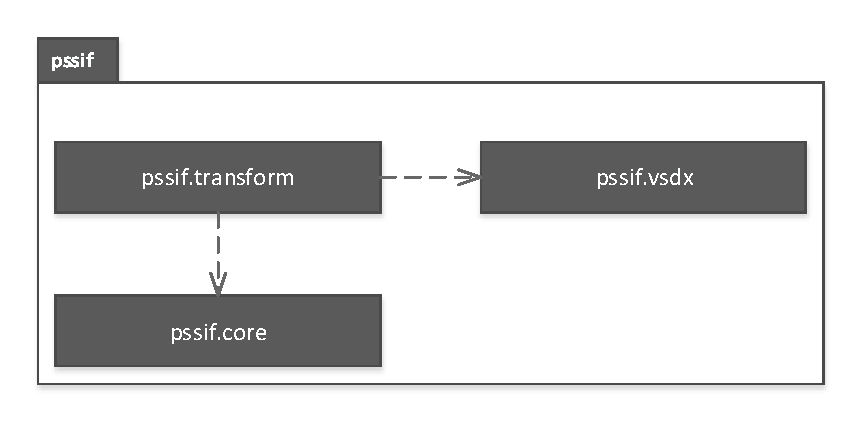
\includegraphics[width=0.8\textwidth]{figures/project-structure.pdf}
\caption{Project Structure}
\label{fig:structure}
\end{figure}

\paragraph{Core} The ''\textbf{core}'' maven module contains the fundamental \gls{api} of the framework. This \gls{api} defines the concepts through which the PSS-IF \gls{dsl} is described, such as Metamodel, Model, NodeTypes, Nodes etc. Furthermore, the core module provides an implementation layer for the concepts of the PSS-IF \gls{dsl}, as well as a number of common utilities, like for example a generator for the canonic PSS-IF Metamodel, as depicted in \figref{fig:canonic}.

\paragraph{Transform} The ''\textbf{transformation}'' maven module provides the \gls{api} used for the definition and execution of transformations, as well as for input and output (I/O) operations. Next to the \glspl{api}, this module also contains their implementation, as well as a number of commonly used helping utilities, concerned with transformation or the serialization to or de-serialization from external formats. Finally, this module contains implementations for the supported source and target languages.

\paragraph{VSDX} The ''\textbf{vsdx}'' module is a dedicated module which provides an API and an implementation for the processing of Microsoft Visio 2013 VSDX documents \cite{ref:visio}. The module defines an abstraction layer describing the structure of a Visio document in an object-oriented fashion, and is used for the serialization and de-serialization of VSDX files.

\section{Components}
\label{sec:impl:components}

After, in the previous section, the coarse-level division of the PSS-IF \gls{poc} parts through maven modules was presented, this section focuses on a more detailed view on the architectural components of the tool. Each of the following subsections describes the function and structure of a specific component of the transformation framework \gls{poc}.

\subsection{Core}

The core is the central component of the framework and is responsible for the realization of key concepts, used for the definition and processing of transformations. The core encloses two major concepts -- those of a \texttt{Metamodel} and a \texttt{Model}, which were already presented in \chapref{chap:approach}.

\subsubsection{Metamodel}

\begin{figure}
\centering
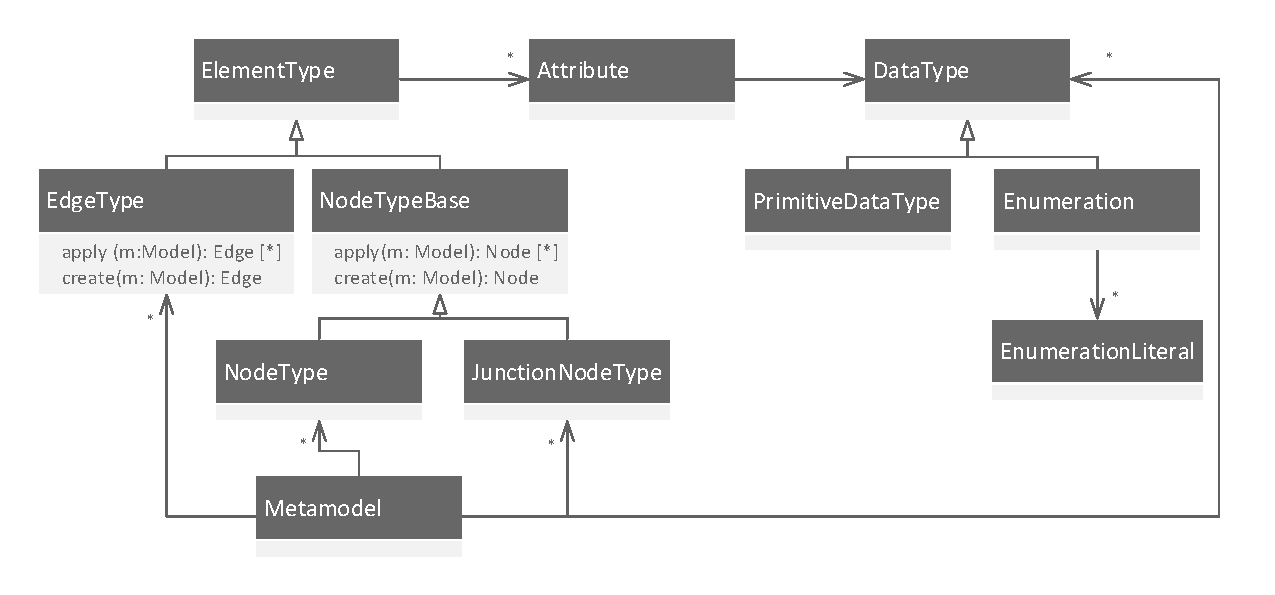
\includegraphics[width=\textwidth]{figures/metamodel.pdf}
\caption{Metamodel API}
\label{fig:metamodel}
\end{figure}

The \texttt{Metamodel} (see \figref{fig:metamodel}) is a concept which enables the users of the framework to define the structure of their data. In this sense, a \texttt{Metamodel} also defines, on the abstract syntax level, the language in which the elements of a PSS-IF \texttt{Model} are described. A parallel in the domain of the \gls{xml} is the \gls{xsd} \cite{ref:xsd}. In essence, a PSS-IF \texttt{Metamodel} is the schema definition in accordance to which a particular \texttt{Model} is created and processed.

A PSS-IF \texttt{Metamodel} captures a number of concepts. In particular, it consists of \texttt{NodeType}s and \texttt{EdgeTypes}, i.e. elements which enable the user to define what kinds of nodes and edges their model may contain, what kinds of features they may have, and how they may relate to each other. Furthermore, in the PSS-IF \gls{poc}, inheritance relations can be defined between both \texttt{NodeType} and \texttt{EdgeType}.

\paragraph{Node Types}

\texttt{NodeType}s are used for the description of the different kinds of nodes in a model and have a number of features. All \texttt{NodeType}s are named and the name must be unique in the scope of all \texttt{NodeType}s and \texttt{EdgeTypes}s within a \texttt{Metamodel}. Furthermore, \texttt{NodeType}s can have a number of attributes, and are connected to other \texttt{NodeType}s over \texttt{EdgeType}s, which can be both incoming and outgoing.

There are two categories of \texttt{NodeType}s -- conventional ones and \texttt{JunctionNodeType}s. The latter actually describe nodes with edge semantics, i.e. they are used for the representation of hyper-edges.

\paragraph{Edge Types}

\texttt{EdgeType}s are used for the description of possible edges in a user's model. \texttt{EdgeType}s also have a name, which is unique in the scope of a \texttt{Metamodel}. For it to be possible to associate the same \texttt{EdgeType} with different pairs of \texttt{NodeType} instances, the concept of a \texttt{ConnectionMapping} is introduced. A \texttt{ConnectionMap\-ping} is an association assigned to a particular \texttt{EdgeType}, which includes an incoming and an outgoing \texttt{NodeType}.

To illustrate the usage of the \texttt{ConnectionMapping}, consider the following example: Assuming two \texttt{NodeType} instances, denoted ''State'' and ''Function'' and an \texttt{EdgeType} ''Control Flow'', which has to connect both node types in both directions. In the PSS-IF \gls{poc} this is achieved by instantiating a single \texttt{EdgeType} ''Control Flow'' and assigning two \texttt{ConnectionMapping} instances to it: one from ''State'' to ''Function'' and one from ''Function'' to ''State''.

\paragraph{Attributes}

For both \texttt{NodeType} and \texttt{EdgeType}, \texttt{Attribute}s can be defined. \texttt{At\-tribute}s are divided into \texttt{AttributeGroup}s, which can be used to separate different kinds of attributes conveniently, for example in a user interface. Furthermore, \texttt{Attribute}s are identified by their names, which have to be unique in the scope of the owning node or edge type. Also, each attribute has a \texttt{DataType}. The PSS-IF \gls{poc} defines a number of primitive data types, like \texttt{String}, \texttt{Integer}, \texttt{Date} and \texttt{Boolean}, and also provides the user with the ability to define custom enumeration data types. Finally, \texttt{Attribute} instances can optionally have a \texttt{Unit} associated with them, which can be particularly useful for numeric attributes. Finally, attributes are divided into categories. Currently, the following categories are defined: \texttt{Monetary}, \texttt{Weight}, \texttt{Density}, \texttt{Time}, \texttt{Geometry}, \texttt{MetaData} and \texttt{Material}.

\paragraph{Inheritance}

As already noted above, for both \texttt{NodeType} and \texttt{EdgeType}, inheritance relations can be defined. When a \texttt{NodeType} inherits from another \texttt{NodeType}, it holds that attribute groups and attributes are inherited from the parent.

\paragraph{Built-In Metamodel Elements}

Every PSS-IF Metamodel has a number of predefined elements. These are the root node and edge types. The root \texttt{NodeType} has the name ''\textbf{Node}'' and provides the following predefined Attributes:

\begin{itemize}
\item \textbf{id}: An identifier of data type \texttt{String} for the node instance of the node type, categorized as Metadata.
\item \textbf{name}: A name of data type \texttt{String}, categorized as \texttt{Metadata}.
\item \textbf{validity start}: A \texttt{Date}, designating the begin of the validity period of the given node, categorized as \texttt{Time}.
\item \textbf{validity end}: A \texttt{Date}, designating the end of the validity period of the given node, categorized as \texttt{Time}.
\item \textbf{version}: The version of the node, of data type \texttt{String}, categorized as \texttt{Metadata}.
\item \textbf{comment}: A comment of the node, of data type \texttt{String}, categorized as \texttt{Meta\-data}.
\end{itemize}

The root \texttt{EdgeType} '''\textbf{Edge}'' has all built-in attributes defined for the root \texttt{NodeType} ''Node'', and also an additional attribute \texttt{directed} of data type \texttt{Boolean} and categorized as \texttt{Metadata}. 

The root node and edge types are also the roots of the inheritance hierarchies for \texttt{NodeType} and \texttt{EdgeType} within a \texttt{Metamodel}. In this sense, any \texttt{NodeType} or \texttt{EdgeType} instance automatically inherits from the respective root type. Thus, it is guaranteed that the set of attributes provided above is automatically defined for all instances of both \texttt{NodeType} and \texttt{EdgeType}. If a node or edge type inherits from a non-root node or edge type, the attributes are inherited transitively, together with all attributes of all ancestors throughout the generalization closure.

\subsubsection{Model}

\begin{figure}
\centering
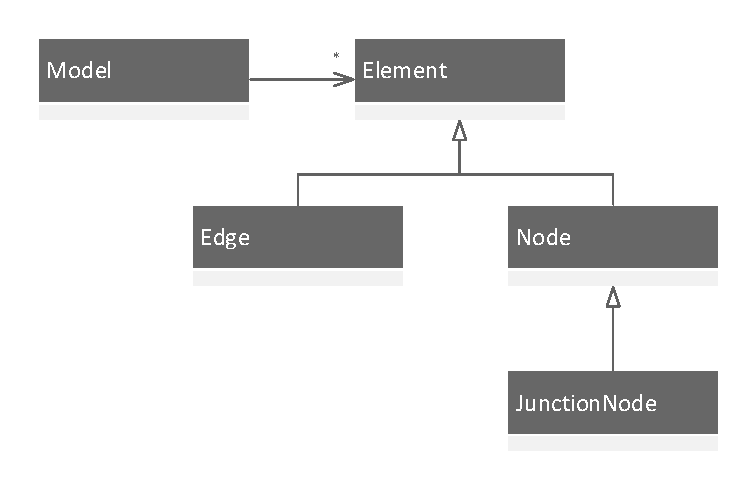
\includegraphics[scale=0.75]{figures/model.pdf}
\caption{Model API}
\label{fig:model}
\end{figure}

The second key component of the PSS-IF \gls{poc} core is the \texttt{Model} (see \figref{fig:model}), which can be seen as a simple graph, consisting of \texttt{Node} and \texttt{Edge} instances. A \texttt{Node} is an ontological instance of a \texttt{NodeType} and an \texttt{Edge} is an ontological instance of the \texttt{EdgeType} of a PSS-IF \texttt{Metamodel}. Note that the elements of the \texttt{Model} are not type-aware themselves and can thus be accessed with different \texttt{Metamodel} instances.

In the PSS-IF \gls{poc} this strategy is used extensively, and a \texttt{Model} does not provide any information or allow any operations itself. All access points to a \texttt{Model} have to be navigated through a \texttt{Metamodel}, i.e. a \texttt{Metamodel} \textit{operates} on a \texttt{Model}. This enables switching between metamodels as the user sees fit, but also to ensure data integrity at all times, by enforcing all modifications to be applied through the \texttt{Metamodel}, which plays the role of the schema for the data contained in the \texttt{Model}.

\subsection{Transformations}

Next to the core, another important component of the PSS-IF \gls{poc} is the transformation \gls{api}. As described in \chapref{chap:approach}, the authors have adopted the ISO 42010 approach, which defines different stakeholders as having different views on their data. Since the utility defines structures on the meta-level, the \gls{poc} describes the views of different stakeholders (source and destination languages) through corresponding Metamodels, called Viewpoints, which perform implicit transformations. For this purpose, viewpoints are defined by the application of a set of transformations to a metamodel.

Thus, the application of a \texttt{Transformation} results in a \texttt{Viewpoint}, i.e. a Metamodel, which modifies the behaviour of the input Metamodel in accordance with the particular kind of transformation applied. As a result, transformations can be applied consequently, each one operating on the result of the previous. A viewpoint is defined in Java as follows:

\begin{verbatim}
Metamodel viewpoint = PSSIFCanonicMetamodelCreator.create();

// create the artificial blocks
viewpoint = new CreateArtificialNodeTransformation
  (state, relationship, block).apply(viewpoint);
viewpoint = new CreateArtificialNodeTransformation
  (function, relationship, block).apply(viewpoint);

// join the informationflow to be created
// between the artificial blocks
viewpoint = new JoinConnectionMappingTransformation
  (informationflow, informationflow.getMapping(state, function),
  new JoinPath(relationship.getMapping(state, block)), block,
  new JoinPath(relationship.getMapping(function, block), block))
    .apply(viewpoint);

// create the artifial controlflow
viewpoint = new CreateArtificialEdgeTransformation
  (informationflow.getMapping(state, function), 
  controlflow.getMapping(state, function)).apply(viewpoint);
\end{verbatim}

\begin{figure}
\centering
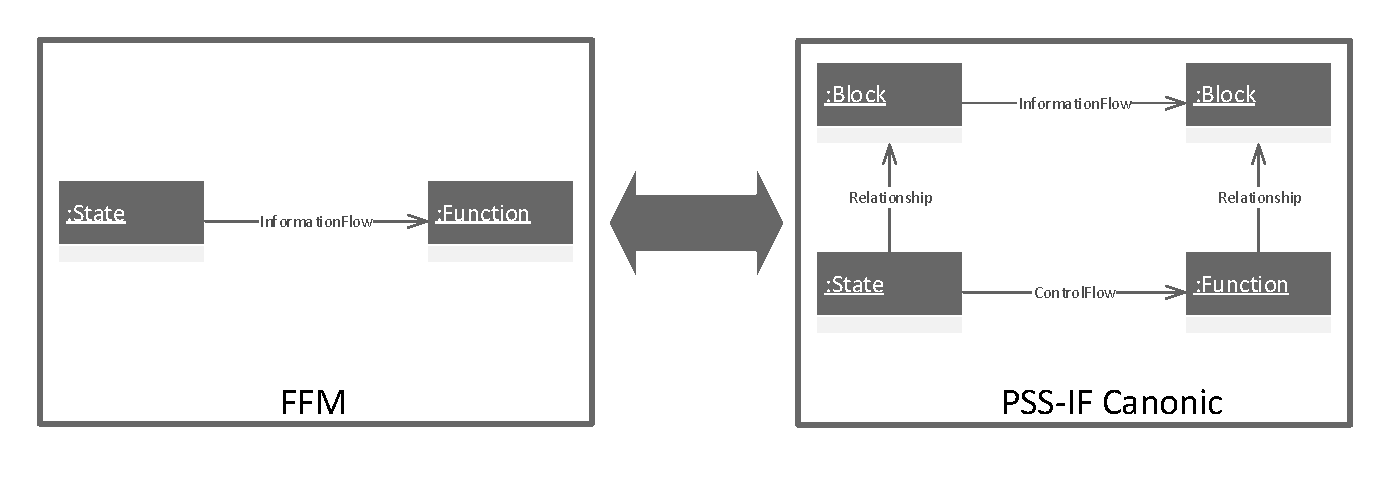
\includegraphics[width=\textwidth]{figures/transformation.pdf}
\caption{Example Transformation}
\label{fig:transformation}
\end{figure}

This viewpoint results in the transformation depicted in \figref{fig:transformation}. Since the behaviour of the \texttt{Viewpoint} is independent of the particular kind of transformation used, the definition of a \texttt{Viewpoint} is reduced to the definition of all necessary transformations and their combination in the appropriate order. The current set of available transformation covers all the ones described in \chapref{chap:approach}.

\subsection{Generic Graph}

A simple component used for intermediate steps in the transformation process is the generic graph component of the PSS-IF \gls{poc}. This component is a simple undirected graph consisting of nodes and edges, which can have string-named attributes with string values, as well as the name of their assumed type. A UML Class Diagram describing the generic graph is depicted in \figref{fig:genericgraph}. In this sense, the graph is an untyped and unstructured equivalent of a PSS-IF Model.

\begin{figure}[h]
\centering
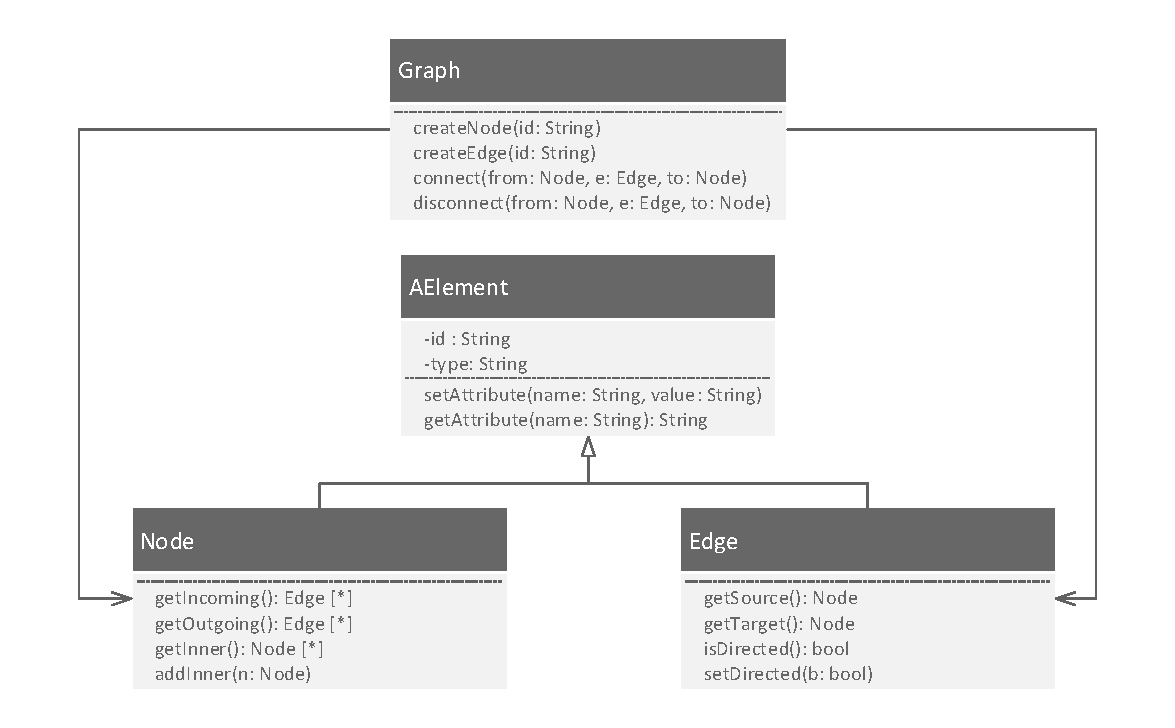
\includegraphics[scale=0.75]{figures/graph.pdf}
\caption{UML Class Diagram of the Generic Graph}
\label{fig:genericgraph}
\end{figure}

In the transformation process, the generic graph is used as an intermediate format, separating the concrete syntax and the abstract syntax of each supported language. The concrete syntax is defined by the file provided by the user and is handled by an \texttt{IoMapper} (see \secref{sec:impl:comp:io}), while the abstract syntax is defined by the \texttt{Viewpoint} and is processed by a \texttt{ModelMapper} (see \secref{sec:impl:comp:model}). The details of the process are provided in \secref{sec:impl:process}.

\subsection{I/O Mappers}
\label{sec:impl:comp:io}

The I/O Mapper component is responsible for the serialization and de-serialization of a generic graph to and from a stream. In this sense, the component has the task to abstract over the concrete syntax used for the representation of the user's data in any particular language. The API of the component is the \texttt{IoMapper} interface, which has the following signature:

\begin{itemize}
\item \texttt{Graph read(InputStream in);}
\item \texttt{void write(Graph graph, OutputStream out);}
\end{itemize}

The same \texttt{IoMapper} may be used for more than one language. For example, the \texttt{VsdxIoMapper} could be used for both, EPC and BPMN.

\subsection{Model Mappers}
\label{sec:impl:comp:model}

The Model Mapper component is responsible for the translation between generic graphs and PSS-IF Models under the provision of a corresponding PSS-IF \texttt{Viewpoint} (Metamodel). In this sense, it handles the translation between the abstract syntax of the external representation and the abstract syntax of the language's viewpoint in PSS-IF. The component is realized through the \texttt{ModelMapper} interface, which has the following signature:

\begin{itemize}
\item \texttt{Model read(Metamodel metamodel, Graph graph);}
\item \texttt{Graph write(Metamodel metamodel, Model model);}
\end{itemize}

In the simplest case, a particular model mapper would simply use the provided viewpoint to directly transfer information between a Model and a graph, processing all nodes, edges and attributes. In more complex cases, pre- or post-processing of the graph may be necessary, to ''normalize'' it into a structure compatible with the viewpoint defined for the particular language (and, hence, with the provided Model). This may, for example, be the case, if the external representation requires the nodes of a graph to be ordered in accordance with a certain rule, or if there are implicit existential dependencies between nodes, implied by the nature of the \texttt{Viewpoint} or a specific \texttt{Transformation}.

In general, it is assumed that one \texttt{ModelMapper} implementation is necessary for each \gls{dsl} to be supported. Theoretically, if the same language is to be imported from or exported to more than one format, and the generic graph is sufficient to express the abstract syntax of both external formats, the same \texttt{ModelMapper} and \texttt{Viewpoint} can be used with different \texttt{IoMapper} implementations, to obtain different serializations of the same data.

\subsection{Microsoft Visio VSDX I/O}

For the serialization and de-serialization of Microsoft Visio 2013 VSDX files needed to support EPC and BPMN, a special component was developed in a dedicated maven module. The component defines an API for the manipulation of VSDX files, operating with the following abstractions:

\begin{itemize}
\item \texttt{VsdxDocument} An object-oriented representation of an entire VSDX document.
\item \texttt{VsdxPage} A page within a VSDX document.
\item \texttt{VsdxMaster} A master shape defined within a VSDX document.
\item \texttt{VsdxShape} A shape, contained either in a page, or in another shape.
\item \texttt{VsdxConnector} A connector shape, i.e. a shape which connects two other shapes.
\end{itemize}

The inter-relation of the different concepts of the VSDX API is depicted in \figref{fig:vsdxapi}.

\begin{figure}[h]
\centering
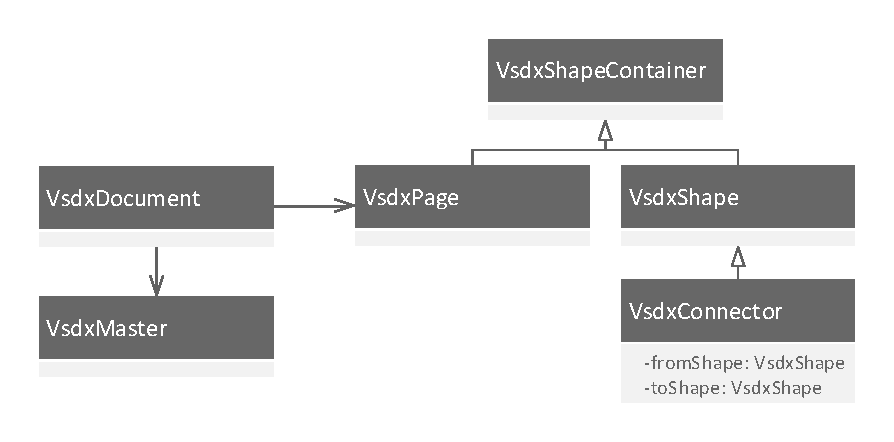
\includegraphics[scale=0.75]{figures/visio.pdf}
\caption{API of the VSDX Component}
\label{fig:vsdxapi}
\end{figure}

It should be noted that the current VSDX component does not provide any mechanisms for layouting, colouring, or other finer operations on a Visio file. This is because the component is aimed explicitly at the extraction and generation of data. The layout of Visio files exported from PSS-IF can be fixed through the usage of algorithms which are built-in in Microsoft Visio. If special decoration of shapes is required, the users can provide their own template files with correspondingly modified master shapes. These template files can then be used in combination with the VSDX component to produce appropriately formatted Visio files. Finally, the API can be extended in future works, to support finer layouting and formatting operations.

\section{Mapping Process}
\label{sec:impl:process}

After, in the previous section, the different components of the PSS-IF \gls{poc} were presented, this section focuses on how the components are tied together and describes the mapping (import and export) process in detail. Here, the term mapping is used, as it covers the processes in both directions and the PSS-IF \gls{poc} implementation handles both cases in the same fashion.

\paragraph{API} The mapping processes are triggered over the corresponding API, represented by the \texttt{Mapper} interface, which has the following signature:

\begin{itemize}
\item \texttt{Model read(Metamodel metamodel, InputStream inputStream);}
\item \texttt{void write(Metamodel metamodel, Model model,}\\ \texttt{OutputStream outputStream);}
\end{itemize}

\paragraph{Implementation} While each specific language, for each file format, requires its own \texttt{Mapper} implementation, the internal procedure for all languages and file formats is the same and is described by the \texttt{AbstractMapper} class, which is the super-class of all \texttt{Mapper} implementations. The \texttt{AbstractMapper} defines the methods of the \texttt{Mapper} API as follows:

\begin{verbatim}
public abstract class AbstractMapper implements Mapper {

 @Override
  public final Model read(Metamodel mm, InputStream in) {
    Graph graph = getIoMapper().read(in);
    Metamodel view = getView(mm);
    ModelMapper modelMapper = getModelMapper();
    return modelMapper.read(view, graph);
  }

  @Override
  public final void write(Metamodel mm, Model m, 
      OutputStream out) {
    Metamodel view = getView(mm);
    ModelMapper modelMapper = getModelMapper();
    Graph graph = modelMapper.write(view, m);
    getIoMapper().write(graph, out);
  }

  protected abstract Metamodel getView(Metamodel metamodel);

  protected abstract ModelMapper getModelMapper();

  protected abstract IoMapper getIoMapper();
 }
\end{verbatim}

As the code above demonstrates, a PSS-IF \texttt{Model} instance is obtained from an external representation by transcoding the external representation into a generic graph, obtaining the \texttt{Viewpoint} of the current language and finally mapping the generic graph to a model in accordance with the viewpoint.

Symmetrically, a file is generated from a PSS-IF \texttt{Model} by first obtaining the \texttt{View\-point} for the current language and using it to translate the model into a generic graph, and then serializing the graph to a stream through the corresponding \texttt{IoMapper}.

\paragraph{Process}

Recall the 6-step process described in \secref{sec:approach:pssif:nutshell}, which describes the transformation process on the conceptual level. In the PSS-IF \gls{poc}, the transformation process is implemented through the consequent invocation of two mappers. The first one is the mapper which de-serializes the source data and transforms it into a Model conforming to the PSS-IF Canonic Metamodel. The second mapper is the one for the target format and is used to write the obtained model into an external representation. For an exemplary source language A and target language B, the Java code describing the transformation process is the following:

\begin{verbatim}
public void transform(Mapper aMapper, Mapper bMapper,
  InputStream inputStream, OutputStream outputStream) {
  
  Metamodel metamodel = PSSIFCanonicMetamodelCreator.create();
  Model model = aMapper.read(metamodel, inputStream);
  bMapper.write(metamodel, model, outputStream);
}
\end{verbatim}

\begin{figure}[h]
\centering
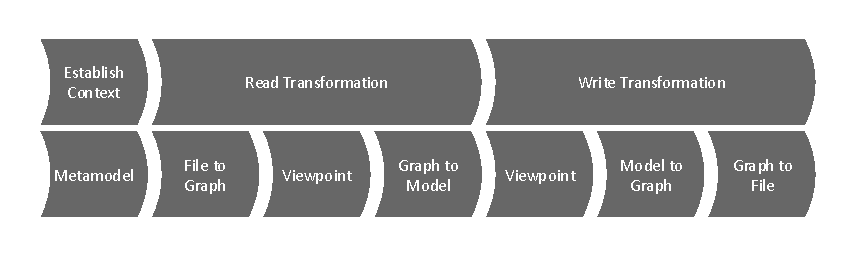
\includegraphics[width=0.8\textwidth]{figures/process.pdf}
\caption{The Transformation Process of the PSS-IF \gls{poc}}
\label{fig:transformationprocess}
\end{figure}

In \figref{fig:transformationprocess}, the transformation process is depicted in two levels of abstraction. The first level addresses the separation into two distinct read and write steps, while the second level demonstrates how both the read and write processes are accomplished by the respective language mappers.

\chapter{Results}
\label{chap:results}

In the previous chapter, the implementation of the PSS-IF \gls{poc} was described. This chapter continues by presenting the results of the interdisciplinary project. In \secref{sec:results:framework} the key features of the PSS-IF \gls{poc}, considered as a framework, are addressed. \secref{sec:results:languages} proceeds with achieved results for each of the four domain-specific languages referenced in \chapref{chap:intro}. Finally, in \secref{sec:results:summary} a brief overview of the results is given.

\section{PSS-IF Proof of Concept}
\label{sec:results:framework}

Throughout the implementation, the authors follow the principles described in \chapref{chap:approach}. Furthermore, the usage of industry-standard libraries and established software-development practices provide for a good long-term manageability of the resulting software. Finally, through the definition of small, simple, yet powerful \glspl{api}, the resulting tool can conveniently be used as a framework to build upon in other projects. The developed \gls{poc} aims at complying to the following software quality attributes:

\paragraph{Generic} The architecture of the implementation defines the transformation process on multiple levels of hierarchy, so that in most cases addition of new features can have a limited impact. Furthermore, divergence from the generic process on each level is possible through the usage of different implementations of the \gls{api} on that level.

\paragraph{Extensible} The clear separation of tasks between components and their collaboration only through well-defined APIs allows new features to be added to each component without intermediate effect on other parts of the software. Also, behind each \gls{api}, implementations can be changed, or new ones can be added, to better fit the needs of the tool's users.

\paragraph{Flexible} Changes in the PSS-IF Canonic Metamodel, or in one of the supported languages can easily be incorporated through adjustment of the metamodel definition and the corresponding viewpoints.

\paragraph{Expressive} Through the adopted meta-modeling approach, the expressiveness of the resulting tool is comparable with that of the Meta-Object Facility (MOF) \cite{ref:mof}, while at the same time being tailored to the set of modeling structures sufficient for the specific field of application.

\paragraph{Accessible} Through the comparatively simple and well-defined APIs, the PSS-IF \gls{poc} can easily be used, once the concepts behind it have been clarified.

\section{Supported Languages}
\label{sec:results:languages}

Through the chosen implementation approach, the objective of transforming models between languages is reduced to the transformation from and to the language defined by the PSS-IF Canonic Metamodel with minimized loss of information. The following sections provide the results for the four languages relevant for this work.

\subsection{Flow-oriented Functional Modeling (FFM)}

Models in the Flow-oriented Functional Modeling (FFM) language can be translated to PSS-IF Canonic. The transferred information is restricted to States and Functions and the Flows between them, as well as the functionary attribute, which is used to forge artificial blocks, or dummy blocks, if no value for this attribute is provided. The original Flow between the States and Functions is then transferred to the artificial blocks, and a ControlFlow is created between the States and Functions. The creation of artificial blocks required the development of the artificialize transformation to create the artificial respectively dummy blocks out of the functionary attribute and the join transformation to transfer the original Flow the additionally created blocks. Furthermore another artificialize transformation is required to create the additional ControlFlow between the States and Functions.

\subsection{Event-Driven Process Chain (EPC)}

Due to their structural similarity, EPC models can be translated into PSS-IF without much difficulty. In the case of this language, the key challenge was the development of an own object-oriented \gls{api} for Microsoft Visio 2013, so that the models can be extracted from and written to VSDX files.

\subsection{Business Process Modeling Notation (BPMN)}

The objective to translate from and to BPMN models described in Microsoft Visio 2013 could not be completed. This is because the BPMN extension of Visio does not use the Visio graph strucuture for the encoding of data, but rather stores the BPMN-specific information into formulae of concrete and abstract nodes. Since the interdisciplinary project has a limited time horizon, the reverse-engineering of this kind of encoding was not possible. 

\subsection{SysML for Mechatronics (SysML4Mechatronics)}

The SysML4Mechatronics is one of the key languages of relevance for the PSS Integration Framework. In the course of the interdisciplinary project, this language presented a challenge, because its original serialization format required a complex multi-phase transformation process, the complexity of which was first realized by the authors during the late phases of the project. Roughly, the phases of the process included the interpretation a UML model encoded in \gls{xmi}, then a \gls{sysml} overlay and finally a special profiling developed by the SFB 768. To overcome this difficulty, the SysML4Mechatronics development team has provided the authors of the interdisciplinary project with an eCore (EMF Meta-Model) description of the SysML4Mecatronics metamodel. With this eCore, SysML4Mechatronics models could be directly mapped to XMI with the \gls{emf}. Thus, \gls{xmi} is the final exchange format adopted for this language in the scope of the interdisciplinary project. Furthermore, the implementation of the SysML4Mechatronics mapper overrides the default mapper strategy by omitting the intermediate step based on a generic graph. This is because both the PSS-IF \gls{poc} and \gls{emf} provide strongly-typed metamodel description facilities. This makes the direct transformation between them simpler and more efficient than a translation through a generic graph where type information has to be lost and re-obtained internally for each element of the model and each of its properties.

\subsection{Canonic Import/Export}

Next to the four domain-specific languages, the PSS-IF \gls{poc} can also import and export the PSS-IF Canonic Model to a GraphML file. This is achieved by using the \texttt{GraphMLIoMapper} with the PSS-IF Canonic Metamodel as a viewpoint.


\section{Summary}
\label{sec:results:summary}

In summary, the interdisciplinary project resulted in a powerful yet flexible solution to the task of transforming between models expressed in different \glspl{dsl}. Adapting the ISO 42010 approach \cite{ref:42010} to documenting software architectures for different stakeholders, a prototype was implemented to support collaboration in the development and operation of \glspl{PSS}. However, the usage of the prototype is not necessarily limited to this domain as it builds on top of a set of generic, atomic transformations which are not domain specific and can easily be reused in different domains. Furthermore the power of the chosen solution was verified by providing viewpoints empowering the prototype to transform from and to two of the four languages in the original objective.
\chapter{Outlook}
\label{chap:outlook}

Having presented the results of the interdisciplinary project, our final contribution is the suggestion of a number of possible improvements to the PSS-IF \gls{poc} in \secref{sec:outlook:improvements}, as well as further developments which could extend the provided \gls{poc} to a central repository used for synchronization along the whole process of developing and operating a \gls{PSS} in \secref{sec:outlook:repo}.

\section{PSS-IF PoC Improvements}
\label{sec:outlook:improvements}

There are a number of possible improvements to the PSS-IF PoC, which would enable the user's to describe even more expressive languages, with better integrity assurance. Some of these are addressed in the following.

\paragraph{ID Handling}

Currently, the handling of identifiers is not part of the tasks of the PSS-IF PoC. A rudimentary artificial ID handling is available in the core, yet it provides no guarantees with regard to the compatibility of the generated IDs in each supported domain-specific language.

\paragraph{Model Edit \gls{api}}

So far, there is no possibility to remove nodes or edges from the model. If the PSS-IF PoC is to be used as the back-end to a user interface, where dynamic behaviour is of importance, these operations might be useful.

\paragraph{Consolidation of Edge Types and Connection Mappings}

In the current implementation the \texttt{ConnectionMapping} interface contains \texttt{apply} methods which are only for internal usage. Since these methods are heavily relied upon by the transformational and can not be removed with reasonable effort, they are for now part of the \gls{api}. However, through the usage of object-oriented patterns it should be possible for a future developer to purge them from the interface without loss of functionality.

\paragraph{Multiplicities}

For certain kinds of edge types, like, for example, the Containment relation, the expressiveness of a metamodel should be increased by adding integrity constraints, such as the possibility that there is at most one container element. Also, certain attributes, for example a hypothetical responsibility, might have more than one value per element.

\paragraph{Acyclicity}

For an edge type, a connection mapping can be defined, which maps from one node type to the same node type. In certain cases, such a self-relationship might, on the semantic level, have to be acyclic. To date, the PSS-IF PoC does not provide a mechanism to specify and ensure this.

\paragraph{Inheritance for Junction Node Types}

Currently, no inheritance rules can be defined for junction node types. While the currently available use-cases do not require such a phenomenon, it might be a future requirement that this is possible.

\section{PSS-IF Repository}
\label{sec:outlook:repo}

The authors consider this work to be a possible foundation for a PSS modeling tool with centralized repository for the management of data and numerous integration interfaces. Many aspects of future research can be addressed along this line of thought, for example a strategy for the merging of models coming from different languages, the evolution and central management of models, as well as the persistence of the central PSS-IF canonic model.

An interesting aspect for future consideration is also the evolution of PSS-IF into a tool used for the interoperability and integration between different modeling tools. In such a case, a number of further languages and syntaxes might have to be supported. Among these are:

\begin{itemize}
\item SysML modelled in Papyrus.
\item EPC modelled in bflow or LibreOffice.
\item BPMN modelled with different Visio stencils or the Eclipse BPMN modeller, ARIS or others.
\item Gliffy used for the drawing of numerous types of diagrams in different languages.
\item Further languages, such as UML State Charts, Sequence or Class Diagrams, or others.
\end{itemize}
%\input{sections/requirements.tex}
%\input{sections/related.tex}
%\input{sections/formal_ql.tex}
%\input{sections/implementation.tex}
%\input{sections/evaluation.tex}
%\input{sections/conclusion.tex}

\appendix
\chapter{Distribution of Tasks}
\label{app:distribution}

This appendix describes the distribution of tasks between the developers of this Proof of Concept (PoC) implementation of the PSS Integration Framework.

\section*{Research}

The research necessary for the development of the PSS-IF PoC was done by both, Bernhard Radke and Konstantin Govedarski.

\section*{Conceptual Development}

The conceptual development of the PSS-IF PoC was done by both, Bernhard Radke and Konstantin Govedarski. Both authors are in comparable knowledge of the concepts and technology behind each component of the PoC system.

\section*{Implementation}

The implementation of the PSS-IF PoC was made by both, Bernhard Radke and Konstantin Govedarski. The approximate distribution of specific tasks is provided below.

\begin{itemize}
\item \textbf{Utilities}: \textit{Bernhard Radke} and \textit{Konstantin Govedarski}
\item \textbf{Core}:
	\begin{itemize}
	\item \textbf{Metamodel}:
		\begin{itemize}
		\item \textbf{Node and Edge Types}: \textit{Bernhard Radke} and \textit{Konstantin Govedarski}
		\item \textbf{Connection Mappings}: \textit{Bernhard Radke}
		\item \textbf{Attributes}: \textit{Konstantin Govedarski}
		\item \textbf{Inheritance}: \textit{Bernhard Radke}
		\end{itemize}
	\item \textbf{Model}: \textit{Bernhard Radke} and \textit{Konstantin Govedarski}
	\item \textbf{Operational API}: \textit{Bernhard Radke}
	\item \textbf{Canonic Metamodel}: \textit{Konstantin Govedarski}
	\item \textbf{Canonic Persistence}: \textit{Bernhard Radke}
 	\end{itemize}
\item \textbf{Transformations}:
	\begin{itemize}
	\item \textbf{Views}: \textit{Bernhard Radke}
	\item \textbf{Operators}: \textit{Bernhard Radke}
	\item \textbf{API}: \textit{Konstantin Govedarski}
	\item \textbf{Generic Graph}: \textit{Konstantin Govedarski}
	\end{itemize}
\item \textbf{Languages and Serialization}:
	\begin{itemize}
	\item \textbf{GraphML}: \textit{Bernhard Radke}
	\item \textbf{EPC (Visio)}: \textit{Konstantin Govedarski}
	\item \textbf{BPMN (Visio)}: \textit{Konstantin Govedarski}
	\item \textbf{SysML4Mechatronics}: \textit{Konstantin Govedarski}
	\end{itemize}
\end{itemize}

\section*{Documentation}

The documentation of the PSS-IF PoC was created by both, Bernhard Radke and Konstantin Govedarski. The documentation includes:

\begin{itemize}
\item This document.
\item The documentation of the source code (JavaDocs).
\end{itemize}
%\input{sections/appendix-owl.tex}

% the bibliography
\bibliography{papers}

\end{document}
